\chapter{Radiactividad y radiación}

A medida que los núcleos se hacen más complejos por el número de partículas que contienen, el tamaño de estos incrementa y, por ende, las fuerzas nucleares se van debilitando mientras que las electrostáticas se incrementan. Esto ocasiona que los núcleos pierdan estabilidad y es por esta razón (aunque no es la única) que la mayor parte de los núcleos pesados presentan radiactividad.

La radiactividad se manifiesta a través de la emisión espontánea de ciertas radiaciones por parte de los núcleos atómicos. Dichas radiaciones son capaces de impresionar placas fotográficas, de producir centelleos o destellos luminosos al incidir en materiales fluorescentes y de producir ionización en los materiales que atraviesan. Estas propiedades sirven de base para la operación de los detectores de las mismas.

\section{Desintegración y tipos de radiaciones}

Una condición para que la desintegración de un núcleo en otros dos ocurra espontáneamente es que la masa del núcleo original sea suficiente para dar lugar a la formación de los núcleos producto y la energía de su movimiento. Si esto no puede suceder espontáneamente, se dice que el núcleo es estable contra la desintegración correspondiente.

Existen tres tipos de radiaciones emitidas por sustancias radiactivas, a las cuales se les asignaron los nombres de radiaciones alfa, beta y gamma en base a sus poderes de penetración crecientes y a sus poderes de ionización decrecientes, respectivamente.

\subsection{Rayos alfa}

Los rayos alfa consisten en dos protones y dos neutrones unidos, formando una partícula de gran masa con carga doblemente positiva y con un gran poder de ionización. Tienen muy corto alcance y, por lo tanto, muy poco poder de penetración.

\subsection{Rayos beta}

Los rayos beta son similares a los electrones en masa y carga. Tienen mayor poder de penetración que los alfa; requieren de varias hojas de aluminio o varios metros de aire para ser contenidos por completo, y su poder de ionización es intermedio.

\subsection{Rayos gamma}

Los rayos gamma son radiaciones electromagnéticas de la misma naturaleza que la luz, que siempre atraviesan cualquier espesor de material absorbente, inclusive el plomo, y producen una ionización relativamente baja.

\section{Actividad de una muestra radiactiva}

La actividad de una muestra radiactiva es el número de desintegraciones que ocurren en la misma por unidad de tiempo; es decir, que la actividad es la rapidez de desintegración de la muestra.

Para medir la cantidad de material radiactivo se usa como unidad el becquerel, que se podría definir como la cantidad de material radiactivo que produce una desintegración por segundo. Sin embargo, la unidad más comúnmente usada para medir actividad es el curie, que se define como la actividad de una muestra en la que ocurren
\[
3.7\times 10^{10}\ \text{desintegraciones por segundo}.
\]

Algunos submúltiplos del curie son:
\begin{align*}
  1\,\mathrm{mCi} &= 1\ \text{milicurie} = 3.7\times 10^{7}\ \text{des/s},\\
  1\,\mu\mathrm{Ci} &= 1\ \text{microcurie} = 3.7\times 10^{4}\ \text{des/s},\\
  1\,\mathrm{pCi} &= 1\ \text{picocurie} = 3.7\times 10^{-2}\ \text{des/s},\\
  1\,\mathrm{Bq} &= 1\ \text{becquerel} = 1\ \mathrm{s}^{-1}.
\end{align*}

\section{Vida media y cálculo de la actividad}

La vida media ($T_{1/2}$) o período de semidesintegración corresponde al tiempo necesario para que la actividad se reduzca a la mitad de su valor inicial.

Para el cálculo de la actividad de una fuente se pueden usar tres métodos.

\subsection{Método analítico}

Se realiza utilizando la siguiente fórmula:
\[
A=A_0e^{-\lambda t},
\]
donde $A$ es la actividad al tiempo $t$, $A_0$ es la actividad original al tiempo $T=0$, $e$ es la base de los logaritmos neperianos ($e=2.71828$), $t$ es el tiempo transcurrido desde que se midió o calculó la actividad original hasta el momento en que se desea calcular la nueva actividad, y
\[
\lambda=\frac{0.693}{\text{vida media}}
\]
es la constante de desintegración.

Supongamos que deseamos calcular la actividad que tendrá el 20 de marzo de 1995 una fuente de Ir-192 que se adquirió el 22 de noviembre de 1994 con 110 Ci. Primero se contabilizan los días transcurridos:
\[
8\ \text{días de noviembre}+31\ \text{de diciembre}+31\ \text{de enero}
+28\ \text{de febrero}+20\ \text{de marzo}=118\ \text{días}.
\]
La vida media del Ir-192 es de 74 días, por lo que:
\begin{align*}
 A &= A_0e^{-\lambda t},\\
 A &= 110e^{-(0.693/74)(118)},\\
 A &= 110e^{-1.105},\\
 A &= 110(0.33),\\
 A &= 36.43\ \mathrm{Ci}.
\end{align*}

\subsection{Método tabular}

Consiste en encontrar el número de días transcurridos desde la fecha de calibración de la fuente hasta la fecha actual y buscar en la tabla (la cual es específica para cada isótopo) el factor que corresponda. Luego se multiplica por la actividad inicial y se obtiene el resultado.

Por ejemplo, para calcular la actividad actual de una fuente con una actividad inicial de 106 Ci, habiendo transcurrido 156 días hasta la fecha de hoy, se toma el factor que más se aproxime a los 156 días; en este caso, 150 días corresponde a un factor de 0.25.
\[
\text{Actividad actual}=0.25\times 106=26.5\ \mathrm{Ci}.
\]

\begin{table}[ht]
\centering
\caption{Tabla de decaimiento para Ir-192.}
\label{tab:decaimiento-ir192}
\begin{tabular}{|c|c||c|c||c|c|}
\hline
\textbf{Días} & \textbf{Factor} & \textbf{Días} & \textbf{Factor} & \textbf{Días} & \textbf{Factor} \\
\hline
25  & 0.79  & 200 & 0.15  & 375 & 0.030 \\
50  & 0.63  & 225 & 0.12  & 400 & 0.024 \\
75  & 0.50  & 250 & 0.096 & 425 & 0.019 \\
100 & 0.39  & 275 & 0.076 & 450 & 0.015 \\
125 & 0.31  & 300 & 0.060 & 475 & 0.012 \\
150 & 0.25  & 325 & 0.048 & 500 & 0.009 \\
175 & 0.19  & 350 & 0.038 & 525 & 0.007 \\
\hline
\end{tabular}
\end{table}

\subsection{Método gráfico}

Consiste en graficar la actividad contra el tiempo, tomando en cuenta que después de cada vida media la actividad original va decayendo a la mitad. Se utiliza papel semilogarítmico para graficarlo; la gráfica es exclusiva para el Ir-192.

\begin{figure}[ht]
  \centering
  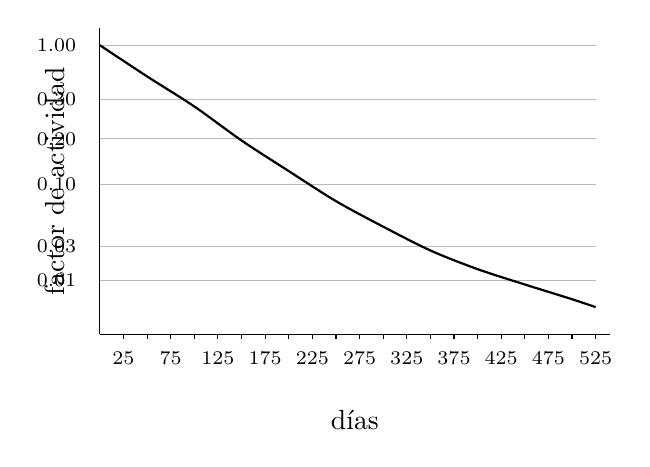
\begin{tikzpicture}[x=0.012cm,y=0.72cm]
    % Réplica vectorial de la gráfica semilogarítmica del manual fuente.
    \draw (0,0) -- (540,0);
    \draw (0,0) -- (0,5.4);
    \foreach \y/\valor in {5.1/1.00,4.15/0.30,3.45/0.20,2.65/0.10,1.55/0.03,0.95/0.01} {
      \draw[gray!55] (0,\y) -- (525,\y);
      \node[anchor=east,xshift=-5pt,font=\scriptsize] at (0,\y) {\valor};
    }
    \foreach \x in {25,50,75,100,125,150,175,200,225,250,275,300,325,350,375,400,425,450,475,500,525}
      {\draw (\x,0) -- (\x,-0.09);}
    % Only alternate ticks carry labels; all ticks remain visible.
    \foreach \x in {25,75,125,175,225,275,325,375,425,475,525}
      {\node[below=3pt,font=\scriptsize] at (\x,0) {\x};}
    \draw[thick] plot[smooth] coordinates
      {(0,5.1) (50,4.55) (100,4.02) (150,3.42) (200,2.88) (250,2.35)
       (300,1.90) (350,1.48) (400,1.15) (450,0.88) (500,0.62) (525,0.48)};
    \node[below=24pt] at (270,0) {días};
    \node[rotate=90] at (-48,2.7) {factor de actividad};
  \end{tikzpicture}
  \caption{Gráfica de decaimiento para Ir-192.}
  \label{fig:grafica-ir192}
\end{figure}
